\chapter{Measurements}

In this chapter we present the various measurements conducted with the
optical setup described in XX.

\section{Intensity Control}

The laser intensity is regulated by a control loop and \gls{aom} in order to
intercept power drifts from the laser source. In this section we want to
discuss the grade of this control loop and estimate an error in subsequent
intensity measures.

\subsection{Long term measurement}

As a start we measured the intensity with a second photodiode over the period
of over \SI{16}{\hour} in an interval of about \SI{2}{\minute}. The measured
intensity timeline is shown in \Cref{fig:intensity_control_long} and the
associated descriptive statistics in \Cref{tab:intensity_control_long}.

\begin{figure}[ht]
  \centering
  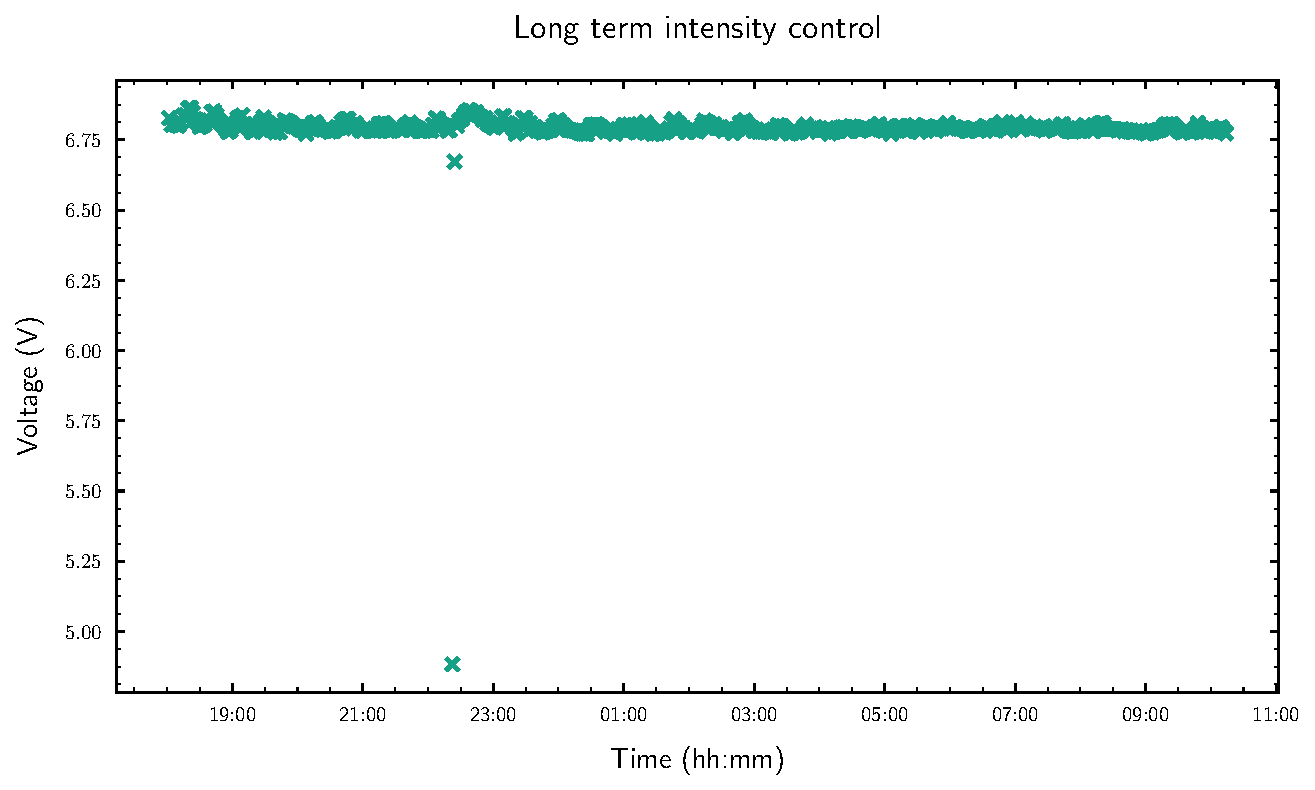
\includegraphics[width=\textwidth]{\figuredir{intensity/control-long.pdf}}
  \captionsetup{width=.8\textwidth}
  \caption{Long term measurement of the intensity with controlled intensity.
    The intensity was measured every \SI{2}{\minute} for over \SI{16}{\hour}
    to determine the accuracy of the intensity controller. The outlier at
    about 22:45 was caused by laboratory visit otherwise the intensity remains
  stable.}
  \label{fig:intensity_control_long}
\end{figure}

We can observe some outliers at about 22:45 which are probably caused by a
late laboratory visit, however we can not assure for a specific reason.

\begin{table}[h]
  \centering
  \begin{tabular}{|c|c|c|c|}
    \hline
    Mean & Minimum & Maximum & Standard deviation \\
    \hline
    \SI{6.79}{\volt} &
    \SI{4.88}{\volt} &
    \SI{6.86}{\volt} &
    \SI{0.09}{\volt} \\
    \hline
  \end{tabular}
  \captionsetup{width=.8\textwidth}
  \caption{Descriptive statistics of the short term measurement of the
  intensity with controlled intensity. Note the small standard deviation.}
  \label{tab:intensity_control_long}
\end{table}

\subsection{Short term measurement}

The previous section gave us already some good insights about the long term
stability of the intensity control loop. Yet in practice typical intensity
measurements are of much smaller magnitude, henceforth it seems close at hand
to measure short term effects too.

\begin{figure}[ht]
  \centering
  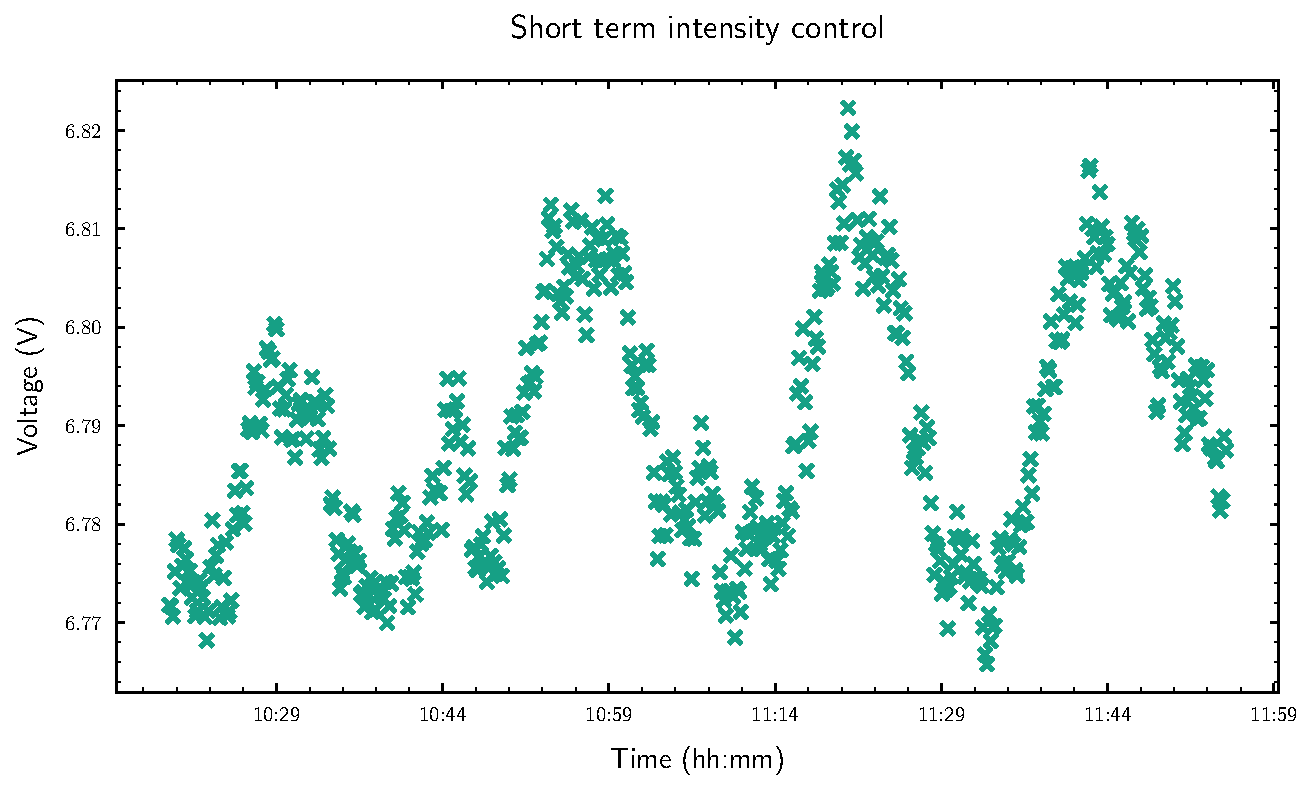
\includegraphics[width=\textwidth]{\figuredir{intensity/control-short.pdf}}
  \captionsetup{width=.8\textwidth}
  \caption{Short term measurement of the intensity with controlled intensity.
    The intensity was measured every \SI{10}{\second} for over \SI{1}{\hour}
    to determine the accuracy of the intensity controller.}
  \label{fig:intensity_control_short}
\end{figure}

For short term measurements we used the same setup as for the long term
measurements. The time parameters now changed to a sample interval of
\SI{10}{\second}. The intensity timeline of the short term measurement is
depicted in \Cref{fig:intensity_control_short} and the associated descriptive
statistics are presented in \Cref{tab:intensity_control_short}.

On a smaller timescale we see that the intensity control loop performs
oscillations. The descriptive statistics show much smaller deviation from
the mean than observed in the long term measurements.

\begin{table}[h]
  \centering
  \begin{tabular}{|c|c|c|c|}
    \hline
    Mean & Minimum & Maximum & Standard deviation \\
    \hline
    \SI{6.78}{\volt} &
    \SI{6.77}{\volt} &
    \SI{6.82}{\volt} &
    \SI{0.01}{\volt} \\
    \hline
  \end{tabular}
  \captionsetup{width=.7\textwidth}
  \caption{Descriptive statistics of the short term measurement of the
  intensity with controlled intensity. Note the small standard deviation.}
  \label{tab:intensity_control_short}
\end{table}

\subsection{Comparison and error estimate}

Even though the previous analysis gave us a good picture of the magnitude
of intensity drifts on different time scale and confirms that the intensity
is in general regulated. Nevertheless we cannot make any statements with
regard to an error estimate without being able to compare the deviation
quantities to actual measurement data.

Because a typical measurement involves \gls{aod} that naturally cause an
intensity difference to the free path configuration we subtracted the
respective mean intensity so the following quantities only account for a
deviation from the respective mean. \Cref{tab:intensity_control} shows the
descriptive statistics of the long and short term measurements of the
intensity control with a typical intensity measurement. Comparing the
standard deviation of short term measurement with the standard deviation of a
typical intensity measurement yields us an approximate error of about
\SI{3}{\percent}. In \Cref{fig:intensity_control} we have the boxplots of
the absolute deviation from the respective mean intensity for the former
three measurement cases to visualize the spread and quantiles of the
intensity.

We conclude that the harmonic noise of the intensity control is in general
small enough to be neglected in further intensity discussion. Nevertheless
the usual intensity drifts may make it difficult to create high-precision
optical potentials.

\begin{table}[h]
  \centering
  \begin{tabular}{|c|c|c|}
    \hline
    Measurement & Value range & Standard deviation \\
    \hline
    long term & \SI{1.98}{\volt} & \SI{0.09}{\volt} \\
    \hline
    short term & \SI{0.06}{\volt} & \SI{0.01}{\volt} \\
    \hline
    typical & \SI{1.43}{\volt} & \SI{0.40}{\volt} \\
    \hline
  \end{tabular}
  \captionsetup{width=.7\textwidth}
  \caption{Descriptive statistics of the short and long term measurement
  of the intensity control and a typical intensity measurements where we
subtracted the mean intensity for comparison.}
  \label{tab:intensity_control}
\end{table}

\begin{figure}[ht]
  \centering
  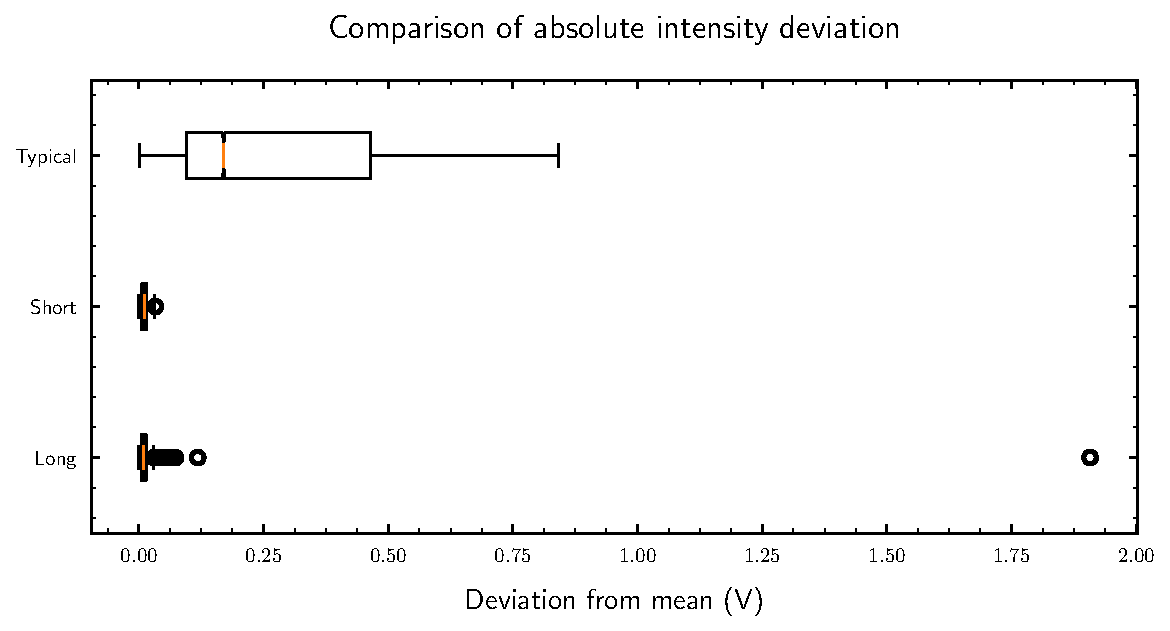
\includegraphics[width=\textwidth]{\figuredir{intensity/control-deviation.pdf}}
  \captionsetup{width=.8\textwidth}
  \caption{Boxplot of the long and short term intensity measurements and a typical
  intensity measurement with the \gls{aod} where we subtracted the mean intensity
  for comparison. The typical measurements covers a much wider intensity range
then deviations from the intensity control loop.}
  \label{fig:intensity_control_comparison}
\end{figure}

\section{Radio frequency signal}

The present section considers the \gls{rf} signal we apply to the
acousto-optic deflectors at different stages of the electronic processing.

\subsection{Signal synthesis}

As already described in the experimental setup section we use \gls{dds} for
signal synthesis. We configure the \gls{dds} to do a linear frequency sweep
from $f_0=\SI{80}{\mega\hertz}$ to $f_1\SI{120}{\mega\hertz}$ as this will be
the later operation range to deflect the laser beam through the \gls{aod}.

\begin{figure}[ht]
  \centering
  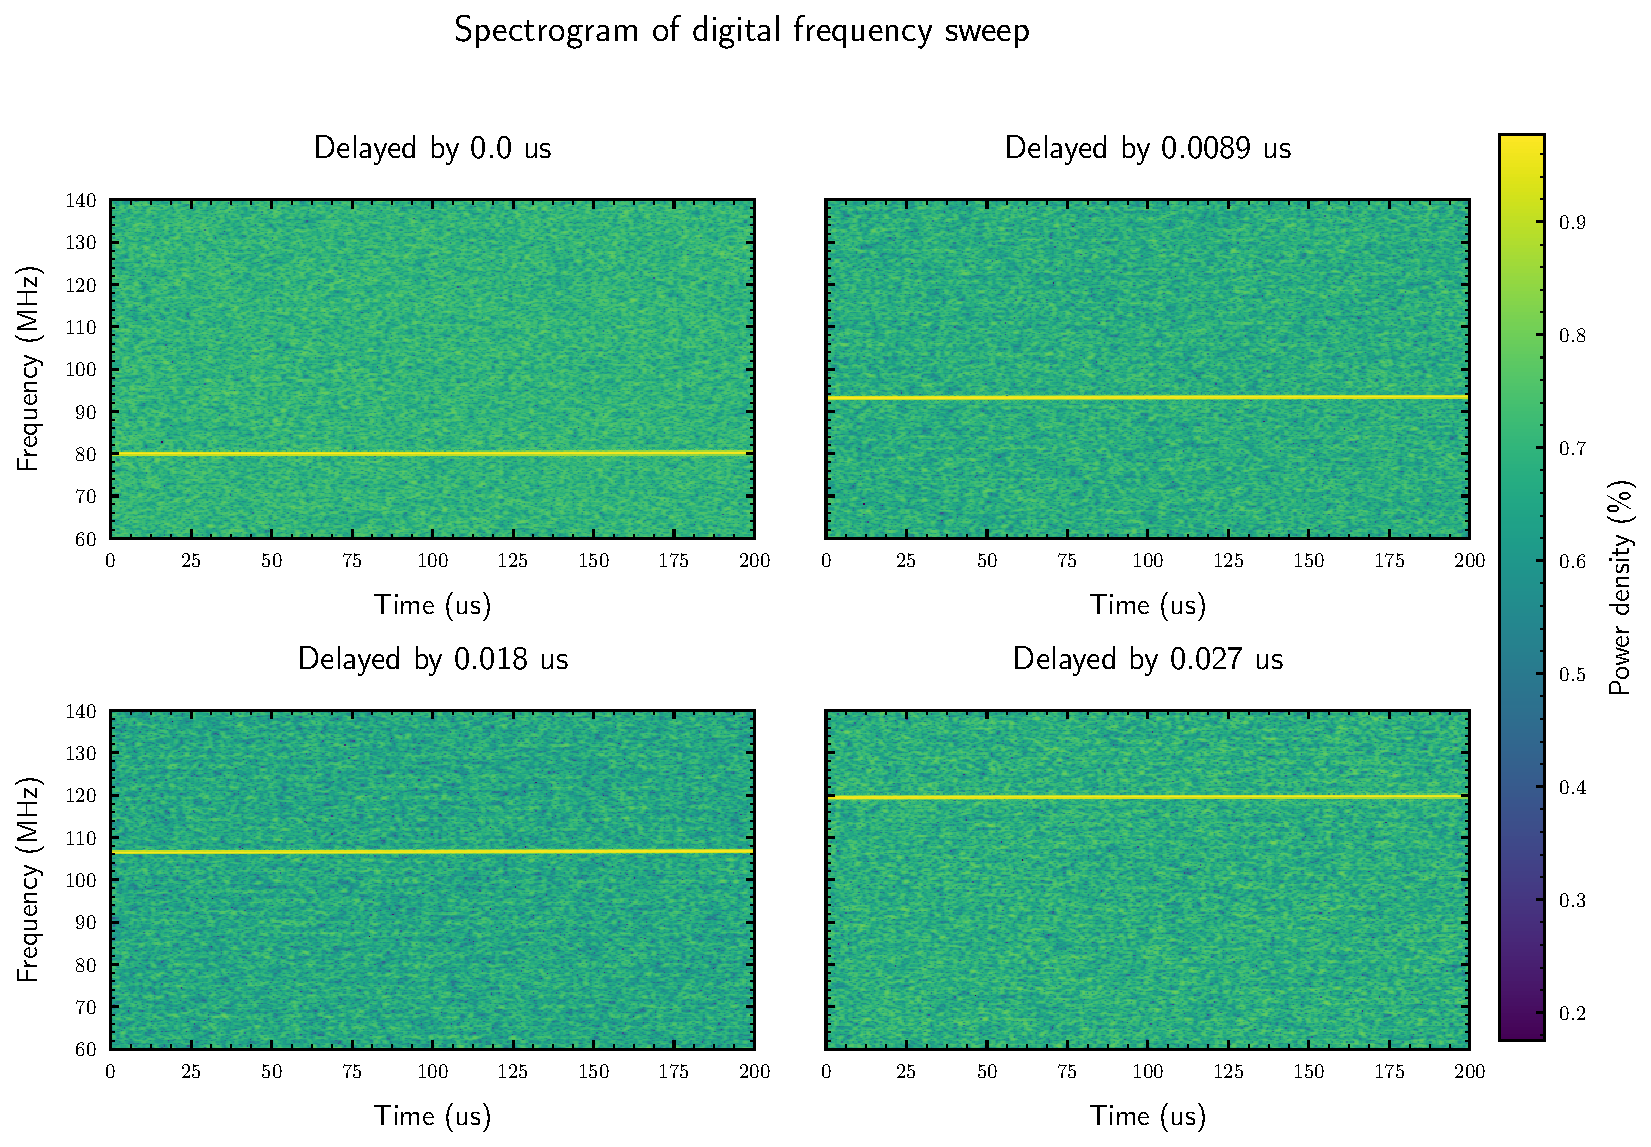
\includegraphics[width=\textwidth]{\figuredir{signal/synthesis/spectrogram.pdf}}
  \captionsetup{width=.8\textwidth}
  \caption{Delayed spectrogram windows of the \gls{dds} output signal in linear
    ramp operation. We see how the frequency starts at $f_0$ and increases
  in discrete steps to the final frequency $f_1$.}
  \label{fig:signal_synthesis_spectrogram}
\end{figure}

At a configured timescale of \SI{10}{\micro\second} the used oscilloscopes
voltage resolution is sufficient for Fourier analysis of the data.
Unfortunately the oscilloscope is not able to capture the complete sweep
period of $T=\SI{26.85}{\milli\second}$. To overcome this obstacle we
inserted a frequency generator between the external trigger source and the
oscilloscope. The frequency generator is configured to emit a square wave
pattern on the rising edge of the external trigger of width $d$. The
oscilloscope was configured to be triggered on the falling edge of the
external trigger signal supplied by the frequency generator. By adjusting
the square wave width $d$ we effectively added a delay to the trigger signal.
In order to capture now the complete signal over duration $T$ we incremented
the delay $d$ in steps of $T/300$. \Cref{fig:signal_synthesis_spectrogram}
shows the spectrogram at four such delays. We observe that because of the
discrete nature of the operation of the \gls{dds} each window only compromises
one distinct frequency that is incremented over the sweep period $T$ in
discrete steps.

\begin{figure}[ht]
  \centering
  \includegraphics[width=\textwidth]{\figuredir{signal/synthesis/frequency-max-amplitude.pdf}}
  \captionsetup{width=.8\textwidth}
  \caption{Maximum amplitude of the two \gls{dds} at different frequencies
  during linear sweep operation. In the two lower curves the \gls{dds} were
configured with enabled inverse sinc filter that is supposed to compensate
frequency dependence in the amplitude.}
  \label{fig:signal_synthesis_frequency_max_amplitude}
\end{figure}

To find the frequency dependence of the amplitude we carried out \gls{fft} to
find the dominant frequency of the signal. Then we collected the maximum
amplitude of each signal window together with the dominant frequency and
visualized the result in \Cref{fig:signal_synthesis_frequency_max_amplitude}.
\Cref{fig:signal_synthesis_frequency_max_amplitude} shows us the maximum
amplitude frequency dependency for different \gls{dds} configurations. We have
used two different \gls{dds} chips as each will later supply a single
\gls{aod}. From \Cref{fig:signal_synthesis_frequency_max_amplitude} we
conclude that there is no difference between distinct \gls{dds}, however we
observe a strong frequency dependence of the amplitude. This behaviour seems
inherent for digital signal synthesis as the \gls{ad9910} comprises an
inverse sinc filter that is supposed to reduce these dependency. From
\Cref{fig:signal_synthesis_frequency_max_amplitude} we see that the effect
of the inverse sinc filter unfortunately only lowers the output amplitude but
does not smooth the frequency dependency.

We summarize that already at the signal source stage a significant frequency
dependency of the output power is introduced that will later have impact on
the effective beam deflection power in the \gls{aod}. Further in our
configuration the inverse sinc filter only lowered the output power, thus
we will keep it disabled for subsequent measurements.

\subsection{Signal amplification}

We now supply the \gls{dds} signal to the amplifier and feed its output
through attentuators to the oscilloscope. For the measurement procedure
we retain the delay window method described in the former section to capture
the complete trace.

\begin{figure}[ht]
  \centering
  \includegraphics[width=\textwidth]{\figuredir{signal/amplification/frequency-max-amplitude.pdf}}
  \captionsetup{width=.8\textwidth}
  \caption{Maximum amplitude at dominant frequency per delayed window for two
  different amplifiers. We can see the discreteness of the frequency domain
from the digital signal synthesis as well as three resonances. Further the
amplifier differ by a constant offset.}
  \label{fig:signal_amplification_frequency_max_amplitude}
\end{figure}

\Cref{fig:signal_amplification_frequency_max_amplitude} presents us the
damped output signal after amplification. Here we can clearly see the finite
frequencies issued by the \gls{dds} as horizontal lines. Further we see that
both amplifiers differ by a constant offset.

\begin{figure}[ht]
  \centering
  \includegraphics[width=\textwidth]{\figuredir{signal/amplification/comparison.pdf}}
  \captionsetup{width=.8\textwidth}
  \caption{Relative amplitude at dominant frequency per delayed window for
  two different amplifiers and their digital signal source. In comparison to
the signal source the amplifiers introduce a further resonance at the
center frequency.}
  \label{fig:signal_amplification_comparison}
\end{figure}

For \Cref{fig:signal_amplification_comparison} we compared the normalized
amplified signals with the normalized signal source. We observe similar
signal shape for both amplifiers. Compared to the signal source frequency
response has changed in that there is an additional frequency response in
between of the two responses of the signal source.

\subsection{Signal reflection}

In the previous section we found.

\begin{figure}[ht]
  \centering
  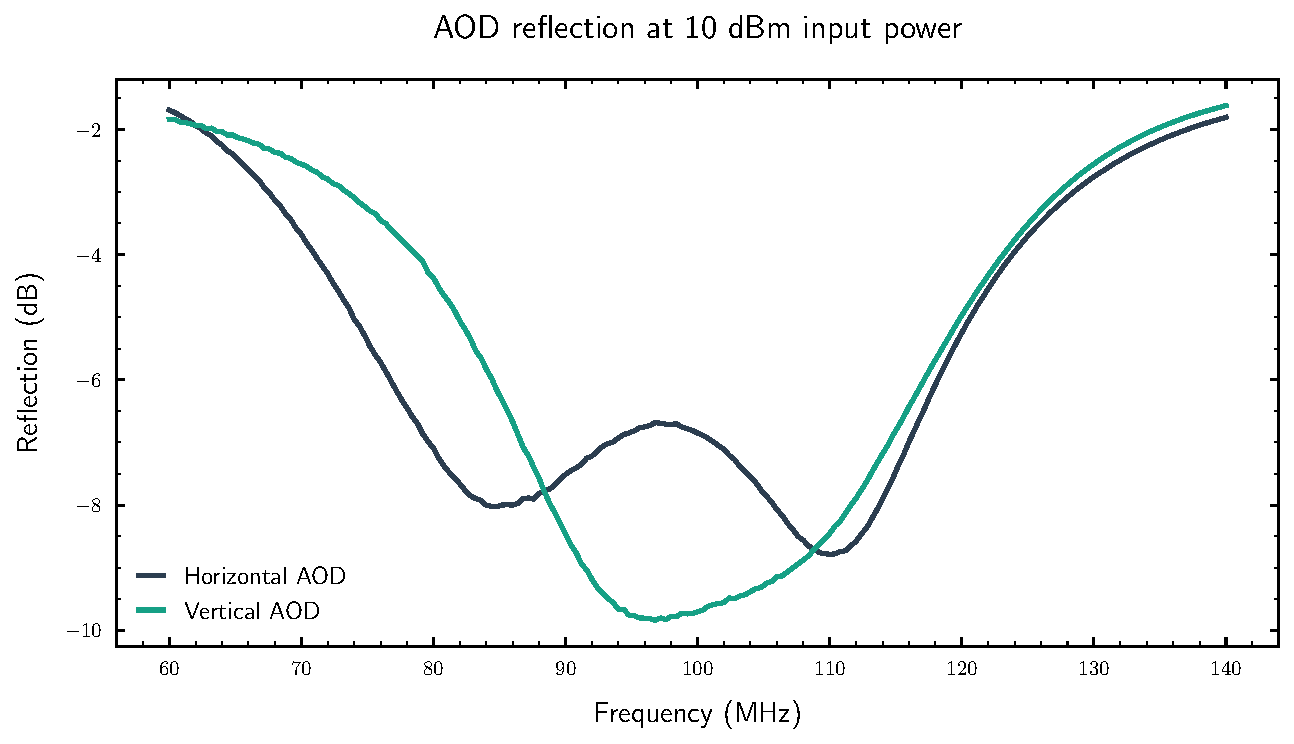
\includegraphics[width=\textwidth]{\figuredir{signal/reflection/direct.pdf}}
  \captionsetup{width=.8\textwidth}
  \caption{We see the signal reflection of the two different \gls{aod} when
  connected directly to the network analyzer. We can see that both crystal
differ in their respective spectrum.}
  \label{fig:signal_reflection_direct}
\end{figure}

\begin{figure}[ht]
  \centering
  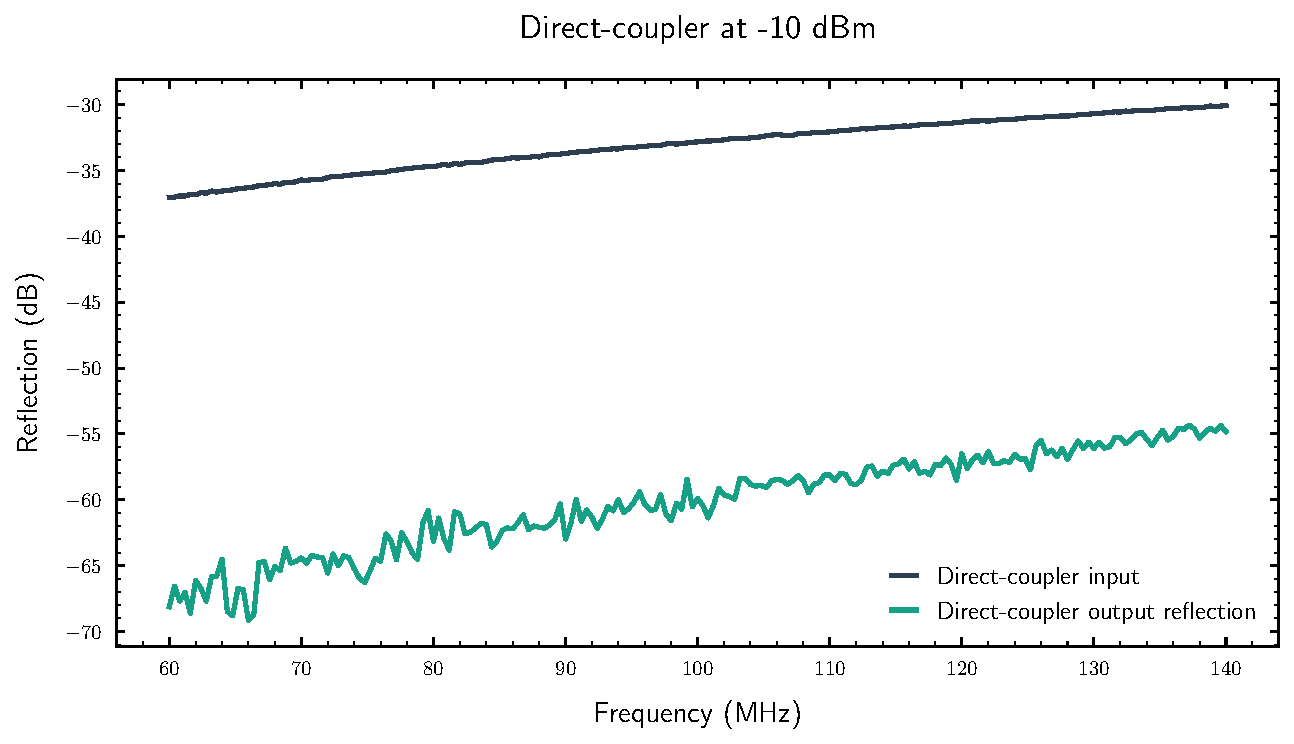
\includegraphics[width=\textwidth]{\figuredir{signal/reflection/coupler.pdf}}
  \captionsetup{width=.8\textwidth}
  \caption{Input power reflection when supplying the direct-coupler with
    \SI{-10}{\deci\bell\meter} input signal and reflection at the output of
    the direct-coupler while other ports are closed with \SI{50}{\ohm}}.
  \label{fig:signal_reflection_coupler}
\end{figure}

\begin{figure}[ht]
  \centering
  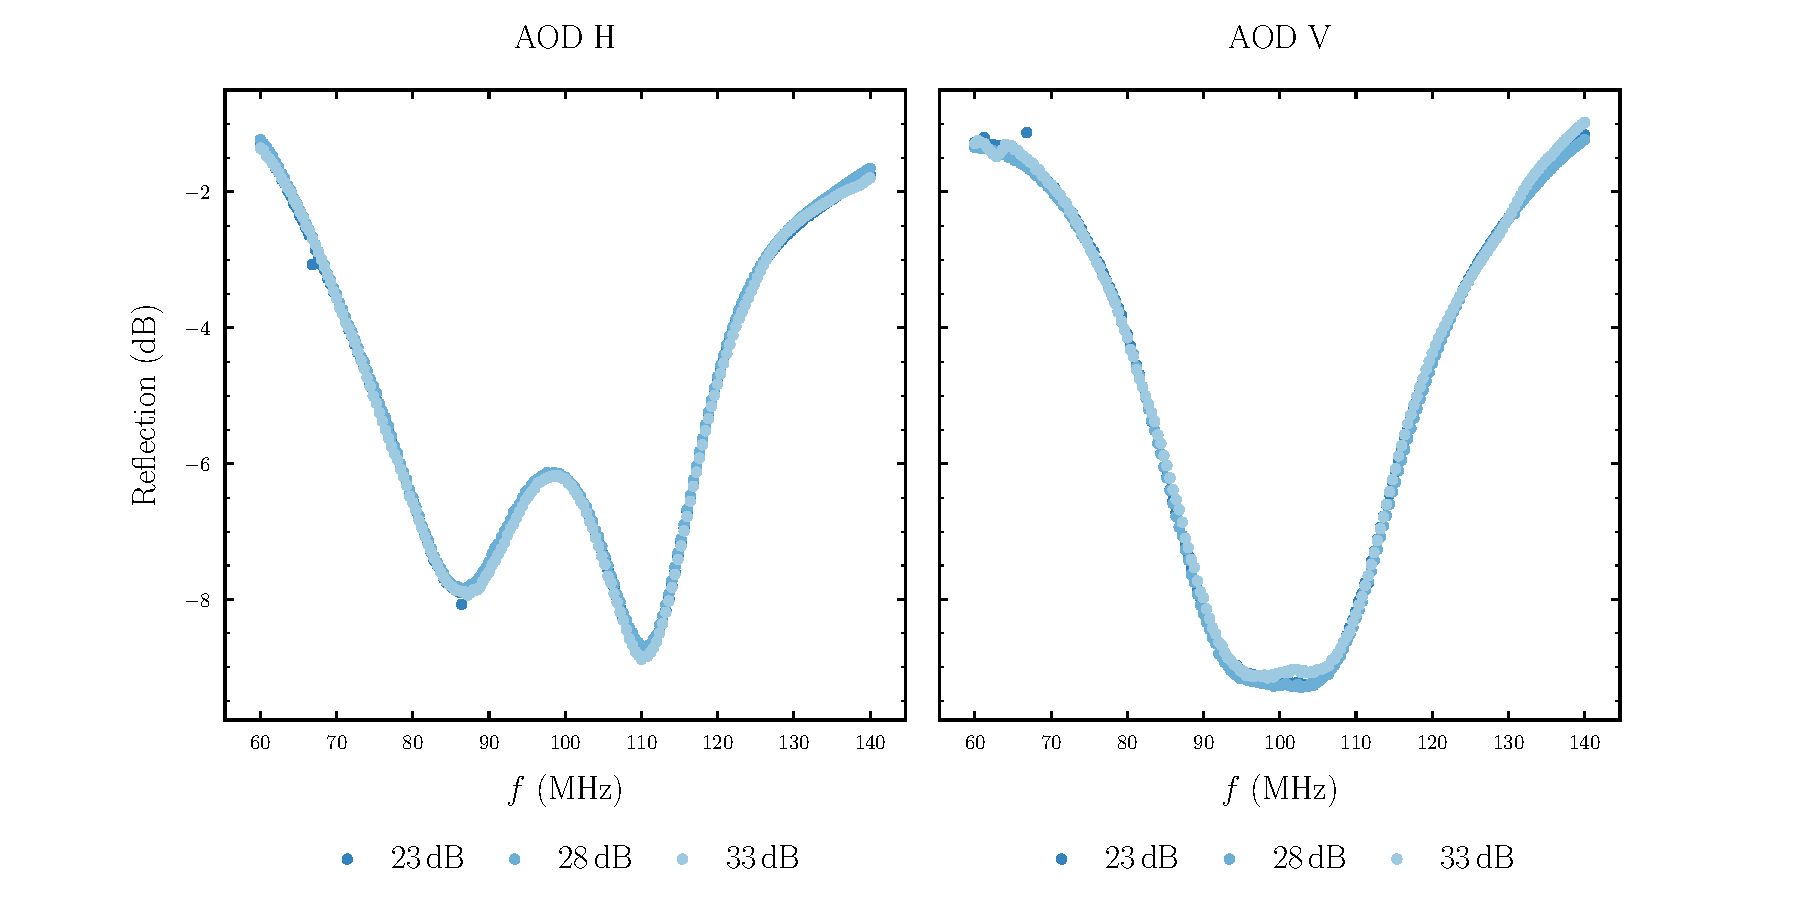
\includegraphics[width=\textwidth]{\figuredir{signal/reflection/coupled.pdf}}
  \captionsetup{width=.8\textwidth}
  \caption{Reflection at the direct-coupler output after amplification of the
  network analyzer input signal for different effective powers. We see that
the applied power does not effect the spectrum.}
  \label{fig:signal_reflection_coupled}
\end{figure}

\begin{figure}[ht]
  \centering
  \includegraphics[width=\textwidth]{\figuredir{signal/reflection/comparison.pdf}}
  \captionsetup{width=.8\textwidth}
  \caption{Comparison of reflection from amplified input signal and direct
  signal provided from the network analyzer. The different reflection spectrum
can be associated to the amplifier.}
  \label{fig:signal_reflection_comparison}
\end{figure}
